\documentclass[12pt,a4paper]{article}
\usepackage[utf8]{inputenc}
\usepackage{amsmath}
\usepackage{amsfonts}
\usepackage{amssymb}

\usepackage{fullpage}
\usepackage{tikz}


\renewcommand\arraystretch{2}

% \usepackage[svgnames]{xcolor} 
\usepackage{listings}

\renewcommand\lstlistingname{Code}

\definecolor{dkgreen}{rgb}{0,0.6,0}
\definecolor{gray}{rgb}{0.9,0.9,0.9}
\definecolor{mauve}{rgb}{1,0.4,0}

\lstset{frame=none,
  backgroundcolor=\color{gray},
  escapeinside={\%*}{*)},
  language=C++,
  aboveskip=3mm,
  belowskip=3mm,
  showstringspaces=false,
  columns=flexible,
  basicstyle={\small\ttfamily},
  numbers=left,
  numberstyle=\tiny\color{black},
  keywordstyle=\color{blue},
  commentstyle=\color{dkgreen},
  stringstyle=\color{mauve},
  breaklines=true,
  breakatwhitespace=true,
  tabsize=3,
  captionpos=b,
  xleftmargin=.25in,
  xrightmargin=.25in
}

%NR specific keywords
\lstset{emph={
    VecDoub,
    MatDoub,
    SVD
    },
    emphstyle={ \color{blue} }   
}

\renewcommand\lstlistingname{Code Segment}

\newcommand{\codeOutput}[1]{\begin{tikzpicture} \node[fill=gray,minimum width=0.921\textwidth,text align=left, text width=0.85\textwidth,text color=black]  at (0,0) {#1}; \end{tikzpicture} }


\begin{document}

\title{Saturn's two Moons\\{\large\emph{Numerical Methods}}}
\author{Nikolaj Iversen and Lukas Schwartz}
\date{April 27th, 2015}
\maketitle


\newpage

%\section{Mathematical Model}
%Find expressions for the elements in the matrix A and the right-hand
%side, say z, for the associated systems of linear equations for the parameters q = (x0; y0; a; b).

The equation for the robot system can be expressed in the form of equation \ref{eq:equationFormat}, where $q = (x_0, y_0, a, b)^T$, as shown in equation \ref{eq:mathematicalModel}.

\begin{equation}
A \cdot q = z
\label{eq:equationFormat}
\end{equation}

\begin{equation}
% -- A --
\left[
\begin{array}{c c c c}
1 & 0 & \cos\left( \theta_1^{(1)}\right)  & \cos\left(\theta_1^{(1)} + \theta_2^{(1)} \right) \\
0 & 1 & \sin\left(\theta_1^{(1)}\right)  & \sin\left(\theta_1^{(1)} + \theta_2^{(1)}\right)  \\
\vdots & \vdots & \vdots & \vdots \\
1 & 0 & \cos\left(\theta_1^{(N)}\right)  & \cos\left(\theta_1^{(N)} + \theta_2^{(N)}\right)  \\
0 & 1 & \sin\left(\theta_1^{(N)}\right)  & \sin\left(\theta_1^{(N)} + \theta_2^{(N)}\right)  \\
\end{array}
\right]
\cdot
% -- q --
\left[
\begin{array}{c}
x_0 \\
y_0 \\
a \\
b \\
\end{array}
\right]
% -- --
=
% -- z --
\left[
\begin{array}{c}
x^{(1)} \\
y^{(1)} \\
\vdots \\
x^{(N)} \\
y^{(N)} \\
\end{array}
\right]
\label{eq:mathematicalModel}
\end{equation}

Where $A$ is a $2 N \times 4$ matrix, $q$ a $4 \times 1$ matrix and $z$ a $2 N \times 1$ matrix.
%
%\section{The SVD Decomposition}
%Read the les with values, insert them in A and compute U, W og
%V using the method from NR. State (with arguments based on the
%SVD matrices) if there are linear dependencies between the parameters
%x0; y0; a; b.

$A$ and $z$ is constructed using code \ref{code:computing_A_z}, this results in the format for $A$ and $z$ as seen in equation \ref{eq:mathematicalModel}.

\lstinputlisting[firstnumber=26,
        firstline=26, 
        lastline=44,
        caption={Computing $A$ and $z$.},
        label={code:computing_A_z}
        ]{../nr_robot/main.cpp}

When computing the SVD using the library supplied by Numerical Recipes, using the data from data set (d1), the matrix in equation \ref{eq:W_and_V_computed} for $W$
% and $V$ are 
is gained.

\begin{equation}
%W
W_{diag} = 
\left[
\begin{array}{c}
23.3788 \\
22.6835 \\
21.8248 \\
21.5074
\end{array}
\right]
%\qquad
%V = 
%\left[
%\begin{array}{c c c c}
%0.589669 & -0.354287 & -0.351603 & 0.634938 \\
%0.311263 & 0.703527 & 0.509408 & 0.385577 \\
%0.493938 & -0.470162 & 0.629460 & -0.372496 \\
%0.558060 & 0.398095 & -0.469743 & -0.556265
%\end{array}
%\right]
\label{eq:W_and_V_computed}
\end{equation}

Where $W_{diag}$ in equation \ref{eq:W_and_V_computed} are the values present in the diagonal of the $4 \times 4$ matrix $W$ from the SVD.

Given that the $W_{diag}$ has four entries, then the rank of $A$ is four. Thus, given $W$ is a $4 \times 4$ matrix of rank four, there are no linear dependencies between $x_0$, $y_0$, $a$ and $b$.
%
%\section{Result and Error Residuals}
Estimate the parameters q = (x0; y0; a; b) and state your results. State
also the residual error Aq - z.
%
%\section{Errors}
%The values of the x(i); y(i)'s are measured with a camera, and there is a
%measurement uncertainty that is estimated to 1mm on each coordinate.
%Estimate the resulting errors on the found parameters using NR, Eq.
%(15.4.19).
The deviation can be found using:
\[
\sigma\left(a_j\right) = \sqrt{ \sum_{i=0}^{N-1} \left( \left( \frac{V_{ji}}{w_i}\right)^2\right) }
\]
This is implemented in Code \ref{code:deviation}.
\lstinputlisting[firstnumber=63,
        firstline=63, 
        lastline=70,
        caption={Computing the deviation.},
        label={code:deviation}
        ]{../nr_robot/main.cpp}

\begin{equation}
\sigma\left(a_j\right) = 
\left[
\begin{array}{c}
 0.044846 \\
 0.044781 \\
 0.044808 \\
 0.044833
\end{array}
\right]
\end{equation}

\section{Saturn's two Moons}
In order to solve the problem of the orbit shift, the Stoerms method is used.
The equations feed to the library are seen in equation \ref{eq:equations_saturn}.

\begin{equation}
\large{
\begin{array}{ll}
\frac{d^2x_1}{dt^2} = - \frac{M g x_1}{r_1^3} + \frac{m_2 g (x_2 - x_1)}{r_{12}^3} &
\frac{d^2y_1}{dt^2} = - \frac{M g y_1}{r_1^3} + \frac{m_2 g (y_2 - y_1)}{r_{12}^3}\\
\frac{d^2x_2}{dt^2} = - \frac{M g x_2}{r_2^3} - \frac{m_1 g (x_2 - x_1)}{r_{12}^3} &
\frac{d^2y_2}{dt^2} = - \frac{M g x_2}{r_2^3} - \frac{m_1 g (y_2 - y_1)}{r_{12}^3}
\end{array}
}
\label{eq:equations_saturn}
\end{equation}

The distance from the moon to Saturn can be seen in figure \ref{fig:distance}.
The crossing point happens about 130 and 530 days.

The phase difference between the two moons is at it's lowest when the moons swap orbit as seen in figure \ref{fig:angle}.

\begin{figure}[h]
\centering
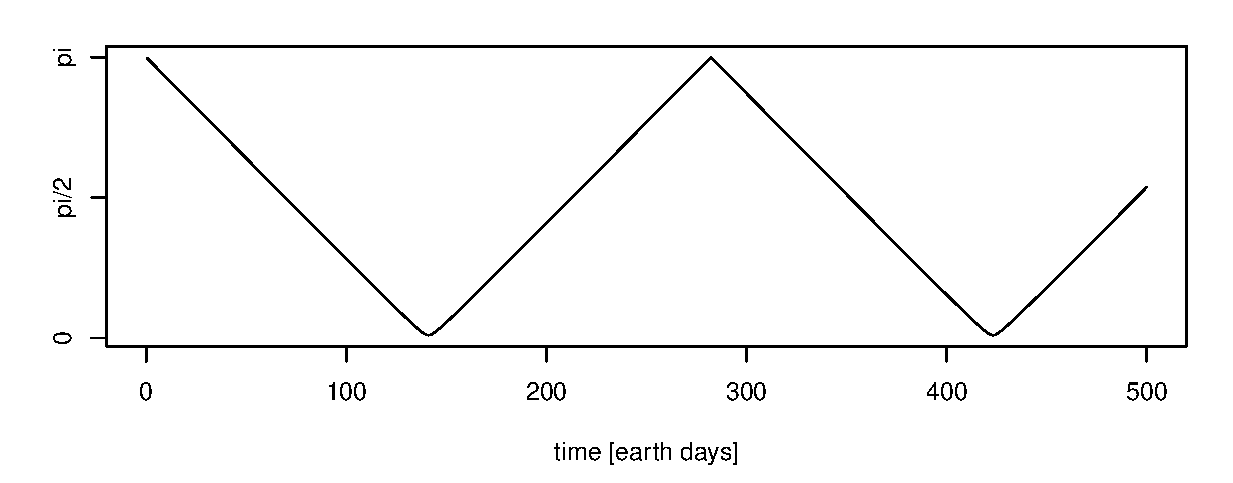
\includegraphics[width=\textwidth]{graphics/angle}
\caption{Absolute phase difference between the two moons.}
\label{fig:angle}
\end{figure}

\begin{figure}[h]
   \centering
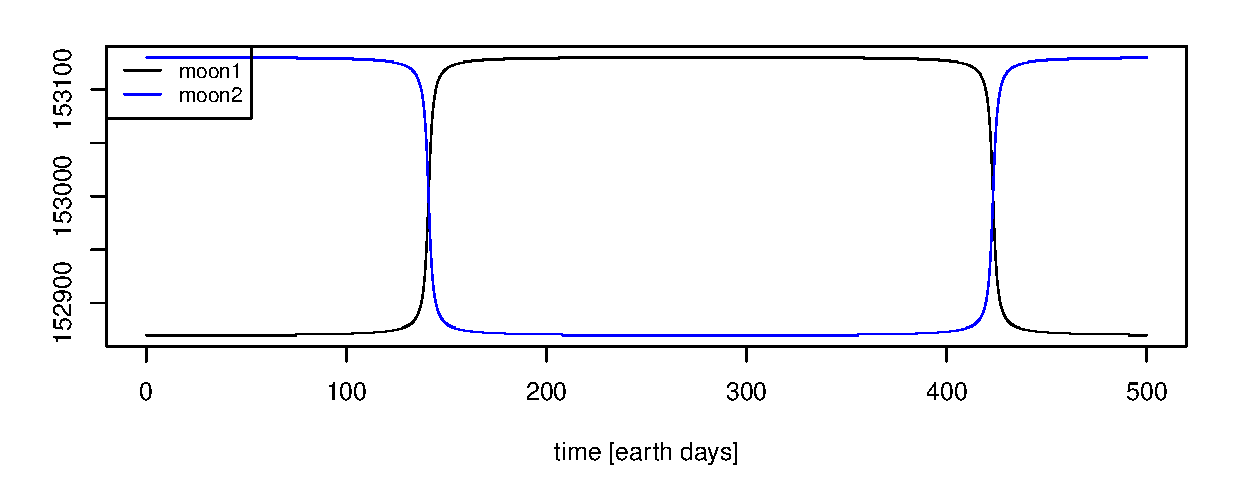
\includegraphics[width=\textwidth]{graphics/distance}
\caption{Distance from the moons to Saturn}
\label{fig:distance}
\end{figure}

The maximum error is predicted using the minimum step size and absolute error per step.
This is done by using the equation \ref{eq:NoSteps}.
Notations are borrowed from the NR library and book.

\begin{equation}
'Max.\ no.\ steps' = \frac{x_2 - x_1}{h_{min}}
\label{eq:NoSteps}
\end{equation}

\(h_{min}\) was set to 0.1 km to avoid too many function-computations.
This gave a maximum number of steps to integrate the function of 5000.
From here, equation \ref{eq:accuracy} can be used to decide the highest accuracy needed to gain a maximum error of 10km.

\begin{equation}
accuracy = atoll \cdot \ 'Max.\ no.\ steps'
\label{eq:accuracy}
\end{equation}

Using the numbers gained earlier the \(atoll\), absolute error for one step, was decided to be \(2\cdot10^{-3}\).

The actual maximum error in the current run is calculated with the StepperStoerm algorithm in NR.
Using that the actual number of iterations of 2931.
The worst case error is 5.862 km.
% Changing a few lines in the NR library gained, the error was output from the step function and passed on to the integrate function.
The stepper function in the NR library calculates the error for each step in order to find the adaptive step size. 
The single step error was summed up and printed.
This gave an global actual error of 1.50603 km. 



\end{document}